\section{Konzept} % Daniel
\begin{frame}
    \frametitle{Konzept}
    \begin{columns}
        \begin{column}{0.4\textwidth}
            \begin{block}{Teilkonzepte}
                \begin{itemize}
                    \item<2-> Korberkennung
                    \item<3-> Ausrichtung
                    \item<4-> Ballbeschleunigung
                    \item<5-> Ballnachführung
                    \item<6-> Kommunikation
                    \item<7-> Energieversorgung
                \end{itemize}
            \end{block}
        \end{column}
        \begin{column}{0.6\textwidth}
            \centering
            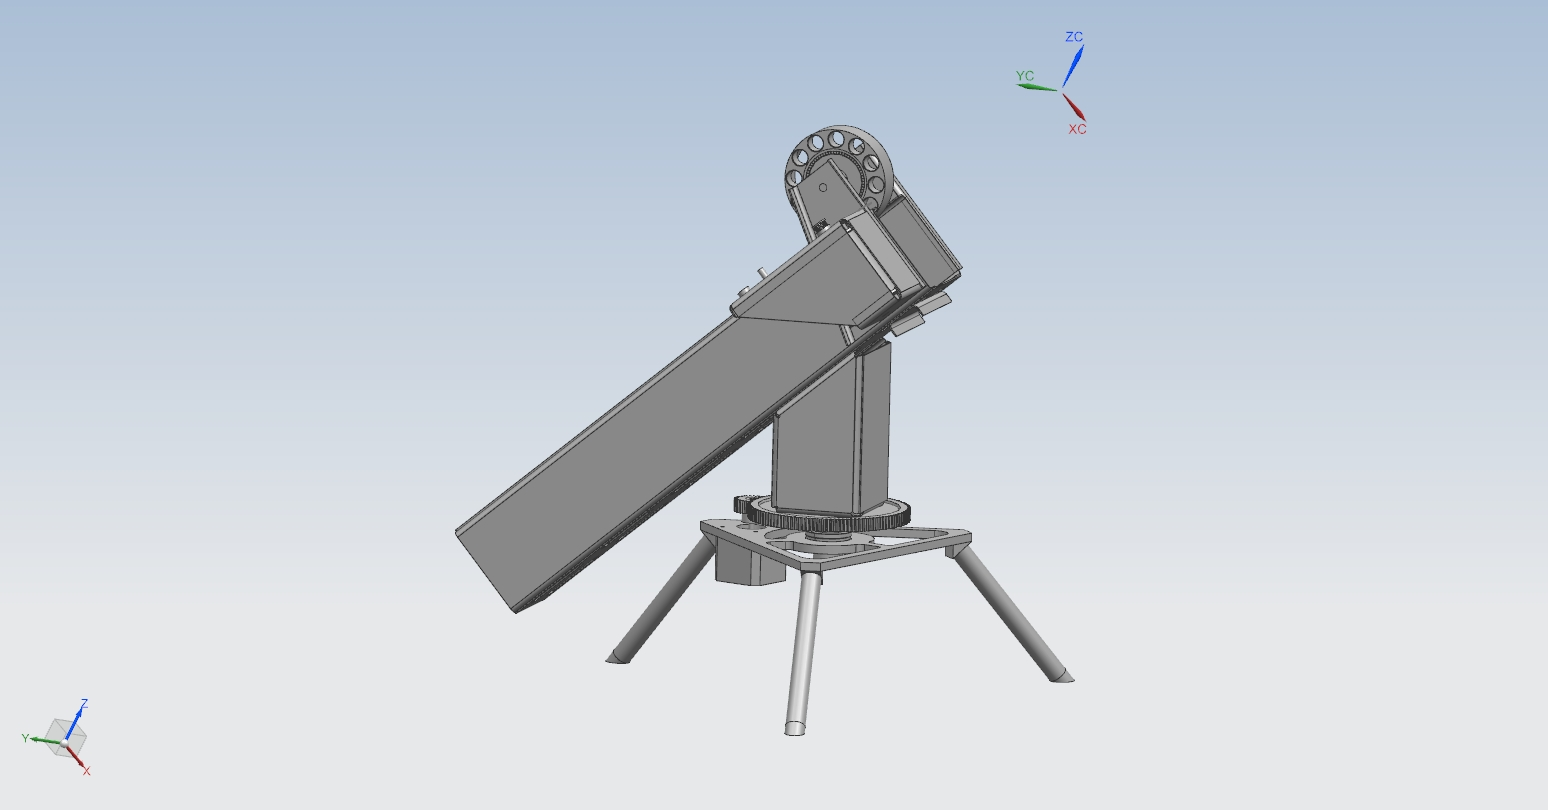
\includegraphics[width=0.8\textwidth, trim = 150mm 50 150mm 10, clip]{../doc/fig/Gesamt_bg1.jpg}
        \end{column}
    \end{columns}
\end{frame}

\begin{frame}
    \frametitle{Konzept}
    \framesubtitle{Korberkennung}
    \begin{block}{Korberkennung}
        \begin{itemize}
            \item Kamera
            \item OpenCV
        \end{itemize}
    \end{block}
\end{frame}

\begin{frame}
    \frametitle{Konzept}
    \framesubtitle{Ausrichtung}
    \begin{block}{Ausrichtung}
        \begin{itemize}
            \item Drehung
            \item Schrittmotor
            \item Getriebe
        \end{itemize}
    \end{block}
\end{frame}

\begin{frame}
    \frametitle{Konzept}
    \framesubtitle{Ballbeschleunigung}
    \begin{block}{Ballbeschleunigung}
        \begin{itemize}
            \item Ein Rad oberhalb
            \item BLDC Motor
        \end{itemize}
    \end{block}
\end{frame}

\begin{frame}
    \frametitle{Konzept}
    \framesubtitle{Ballnachführung}
    \begin{block}{Ballnachführung}
        \begin{itemize}
            \item Stahlband
            \item DC Motor
        \end{itemize}
    \end{block}
\end{frame}

\begin{frame}
    \frametitle{Konzept}
    \framesubtitle{Kommunikation}
    \begin{block}{Kommunikation}
        \begin{itemize}
            \item Bluetooth für Steuerung
            \item WLAN für Kamerabild
        \end{itemize}
    \end{block}
\end{frame}

\begin{frame}
    \frametitle{Konzept}
    \framesubtitle{Energieversorgung}
    \begin{block}{Energieversorgung}
        \begin{itemize}
            \item Netzteil
            \item 24 \ldots 36 V
        \end{itemize}
    \end{block}
\end{frame}

